\chapter{RISC-V \ SOC设计}\label{chap:soc}

由于神经网络中的卷积计算、池化计算及全连接计算等都在加速器中完成,而网络中的图像预处理、softmax层计算等耗时较短的操作则由 RISC-V 处理器来完成。为了让 CNN 加速器和 RISC-V 处理器协同工作,在本章中我们设计了一个通用的 SOC,将 CNN 加速器作为 RISC-V 处理器的一个外设,由 RSIC-V 处理器进行流程控制和图像预处理、softmax层计算等工作,CNN 加速器负责主要的卷积神经网络计算任务。为了提高设计效率,本设计中将 RISC-V 处理器和神经网络加速器封装成带有 AXI4 总线接口 的 IP,通过 AXI4 总线与 UART、GPIO、定时器等外设连接。下面详细介绍 SOC 的设计过程。

\section{SOC 整体设计}

由于目前 RISC-V 基金会还没有发布标准的 RISC-V 调试架构文档\citep{胡振波2018手把手教你设计},因此目前开源的几款 RISC-V 处理器大多不带调试机制,这就给软件调试带来了不便之处,为此这里参考了 PYNQ MicroBlaze Subsystem 的设计 \citep{PYNQ_MB},在 ZYNQ 芯片上运行 Linux 系统与 RISC-V 处理器共享内存来完成程序的下载过程。

\begin{figure}[!htbp]
    \centering
    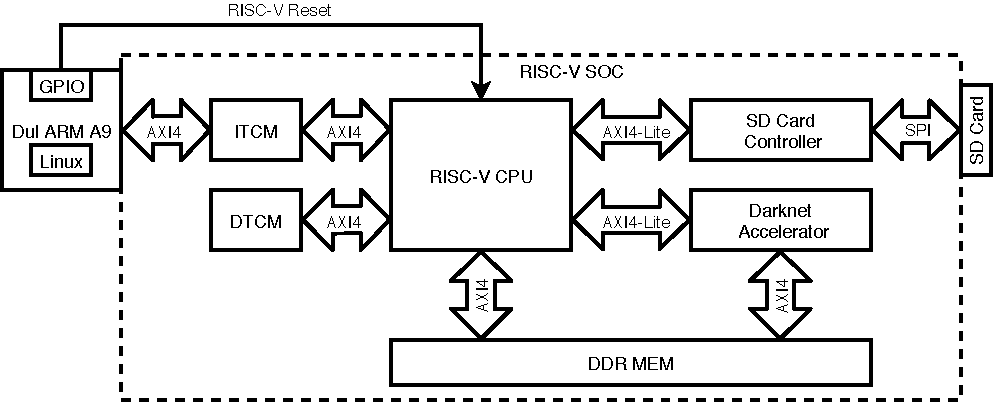
\includegraphics[width=0.80\textwidth]{soc}
    \caption{RISC-V SOC 架构}
    \label{fig:soc}
\end{figure}

SOC 整体的结构设计如图~\ref{fig:soc}所示。在本设计中,将 SOC 部分在 ZYNQ 的 PL 部分实现。RISC-V 的 ITCM 使用一个双端口 Block RAM 实现,ITCM 的一个端口与 RISC-V 处理器连接,其另一个端口通过 AXI4 总线与 ZYNQ 上的 ARM 核相连,ARM 核可以读写这块 ITCM 中的数据。在 ZYNQ 的 双核 ARM A9 上运行 linux 系统,在该系统上使用交叉编译工具编译 RISC-V 的软件程序,将编译后的二进制文件放入 RISC-V 处理器的 ITCM 中,再复位 RISC-V 处理器,便可以使 RISC-V 处理器执行相应的程序。

% \section{RISC-V 处理器选择}

% \# 需要各 RISC-V 处理器的性能数据对比。

\section{SOC 硬件详细设计}

本 SOC 主要包含 RISC-V 处理器,集成 ROM、RAM,包含了基本的外设(包括GPIO、UART等)以及神经网络加速器,各模块之间通过 AXI4 总线连接。

\subsection{RISC-V处理器接口描述}
Ibex处理器的结构如图~\ref{fig:blockdigram}所示,Ibex处理器的接口主要包含6个部分:

\begin{figure}[htbp]
    \centering
    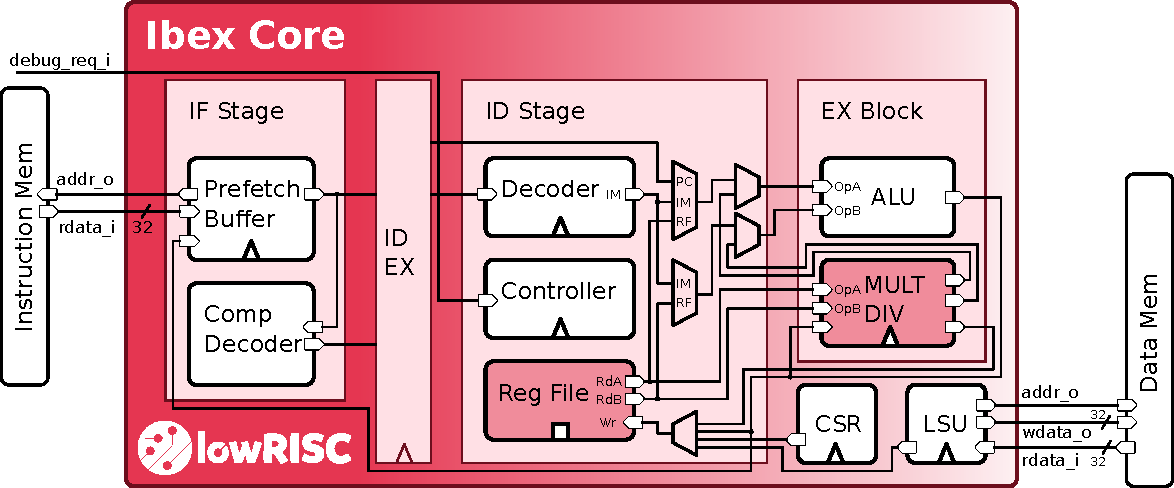
\includegraphics[width=0.9\textwidth]{blockdigram}
    \caption{Ibex处理器结构}
    \label{fig:blockdigram}
\end{figure}

\begin{enumerate}
    \item 时钟和复位接口;
    \item 控制接口;
    \item 指令私有总线接口;
    \item 数据私有总线接口;
    \item 中断接口;
    \item Debug接口。
\end{enumerate}

%\subsection{私有总线转AHB总线}
%由于Ibex使用的是私有总线,而本SOC平台的为了保证通用性,使用的是AMBA总线,因此需要将Ibex私用总线转换为AMBA总线。
%Ibex私有总线时序如图\ref{fig:ibexsx}所示:
%
%\begin{figure}[htbp]
%   \centering
%   \includegraphics[width=\textwidth]{ibex私有总线时序}
%   \caption{Ibex私有总线时序}
%   \label{fig:ibexsx}
%\end{figure}
%
%AHB总线的时序如图\ref{fig:ahbsx}所示:
%
%\begin{figure}[htbp]
%   \centering
%   \includegraphics[width=\textwidth]{AHB总线时序}
%   \caption{AHB总线时序}
%   \label{fig:ahbsx}
%\end{figure}

\subsection{SOC片上存储资源}
本SOC中的片上存储器资源分为ITCM和DTCM,其结构如图~\ref{fig:sram} 所示。其中 ITCM(Instruction Tightly Coupled Memory)为 RISC-V 处理器内核私有的指令寄存器,其大小可以配置,默认设置为 64Kb;默认的起始地址是 0x8000\_0000;由于 ITCM 是用来存放指令的,所以 RISC-V 处理器在正常运行时,这块区域是只读的,为了实现程序的掉电保存,需要将程序存放在外置的非易失性存储器上,在处理器复位后,使用 Load 和 Store 指令将程序搬运到 ITCM 中,这个阶段 ITCM 为可读写状态。因此 ITCM 使用一个双端口 Block RAM 实现,其有两个读写接口,一个读写接口直连处理器的指令总线接口,另一个接口通过一个仲裁器分别连接了处理器的数据总线接口和Debug模块的数据接口。

DTCM(Data Tightly Coupled Memory)为 RISC-V 处理器内核私有的数据存储器,其大小可以配置,默认为 64Kb;默认的起始地址是 0x9000\_0000;DTCM 用来存放程序运行中的数据,相当于处理器的内存,因此在通常状态下,DTCM 都是可读写的,所以 DTCM 使用一个单端口 RAM 实现,其接口直接连接在处理器的数据总线接口上。

\begin{figure}[htbp]
    \centering
    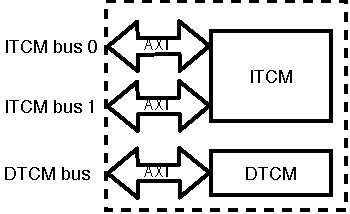
\includegraphics[width=0.4\textwidth]{sram}
    \caption{片上存储器资源结构框图}
    \label{fig:sram}
\end{figure}

% \begin{enumerate}
%     \item 大小可配置,默认设置为64Kb;
%     \item 可配置地址区间,默认起始地址为0x8000\_0000;
%     \item ITCM虽然主要用来存放指令,但是其地址区间也可以被处理器核的Load和Store指令访问,从而实现将存储在片外存储器上的指令加载到片内ITCM上,实现程序的掉电保存。
% \end{enumerate}

% DTCM为RISC-V处理器内核私有的数据存储器,其特性如下:
% \begin{enumerate}
%     \item 大小可配置,默认设置为64Kb;
%     \item 可配置地址区间,默认起始地址为0x9000\_0000;
%     \item DTCM只能被处理器的数据存储器访问指令访问,因此只能用来存放数据。
% \end{enumerate}

% ITCM使用一个双端口RAM实现,其有两个读写接口,一个读写接口直连处理器的指令总线接口,另一个接口通过一个仲裁器分别连接了处理器的数据总线接口和Debug模块的数据接口。

% DTCM使用一个单端口RAM实现,其接口直接连接在处理器的数据总线接口上。

\subsection{SOC外设资源}
\begin{enumerate}
    \item UART 

    本SOC中实现了一个URAT外设,采用 AXI Lite 总线接口,结构如图~\ref{fig:uart} 所示。该 UART 在接收端使用 16 倍波特率的采样频率进行采样;数据格式为 8 位数据,没有奇偶校验位,1 位起始位,1 位停止位;波特率由内部寄存器控制,支持软件调节;支持全双工的接收和发送数据,内部带有接收缓存和发送缓存;中断产生的阈值由内部寄存器控制,支持软件调节。
    
    \begin{figure}[htbp]
        \centering
        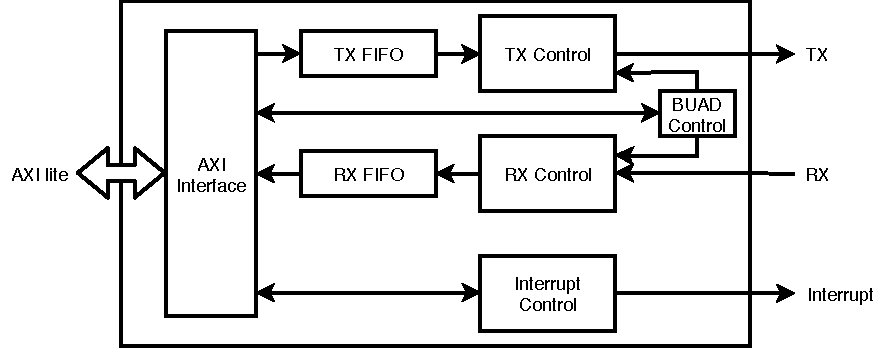
\includegraphics[width=0.7\textwidth]{uart}
        \caption{UART结构框图}
        \label{fig:uart}
    \end{figure}
    
    % \begin{itemize}
    %     \item 支持发送和接收数据能力;
    %     \item 支持8-N-1数据传输格式:即8位数据位、没有奇偶校验位、1位起始位、1位停止位;
    %     \item 支持软件可编程的阈值产生中断;
    %     \item 支持软件可编程的波特率调节;
    %     \item 在接收端采用16倍波特率的采样频率进行采样接收数据。
    % \end{itemize}
    
    \item GPIO
    
    本SOC中实现了一个双通道 32 位GPIO,采用 AXI Lite 总线接口,其结构如图~\ref{fig:gpio} 所示。每个通道有 32 位的双向 I/O 口,每位 I/O 口的方向由内部寄存器控制,支持软件调节;内部带有一个中断控制器,在 I/O 口为输入时,可以产生中断信号。
    
    \begin{figure}[htbp]
        \centering
        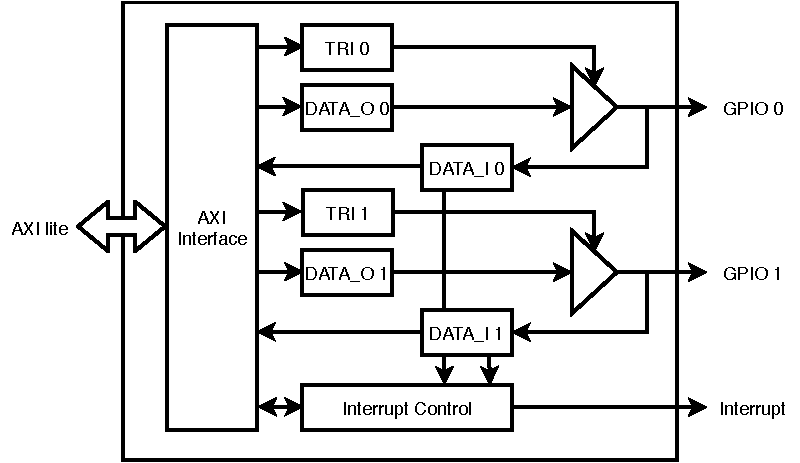
\includegraphics[width=0.7\textwidth]{gpio}
        \caption{GPIO结构框图}
        \label{fig:gpio}
    \end{figure}
    
    % \begin{itemize}
    %     \item 每个GPIO控制器提供一组32个I/O的通用输入输出接口;
    %     \item 每个I/O均可直接接受软件编程的可配置寄存器控制,此时I/O的表现为输出;
    %     \item 每个I/O均可直接接受硬件接口控制信号,此时I/O表现为输入;
    %     \item 每个I/O均可产生中断。
    % \end{itemize}
    
    \item RTC
    
    RTC(Real-Time Clock)是MCU中常用的模块,用于给程序运行提供精确计时的功能。本 SOC 中设计了一个 RTC 模块,其结构如图~\ref{fig:rtc} 所示。本设计中的 RTC 包含了两个独立的 32 位计数器,其触发信号为 CPU 的时钟,这两个计数器可以在其内部寄存器的控制下级联成一个 64 位的计数器。计数器的初始值可由内部寄存器控制,计数器向上计数,加满之后再加一,就会产生溢出,从而通知中断控制器产生中断。
    
    \begin{figure}[htbp]
        \centering
        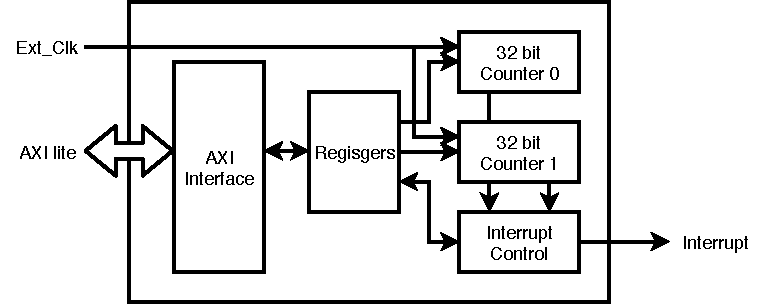
\includegraphics[width=0.7\textwidth]{rtc}
        \caption{RTC结构框图}
        \label{fig:rtc}
    \end{figure}
    
    % \begin{itemize}
    %     \item RTC本质上是两个独立的32位计数器,计数器在被使能后每个周期自增加一;
    %     \item 两个独立的RTC受软件编程控制可级联为一个64位计数器;
    %     \item 支持可编程寄存器设定计数器的比较阈值,一旦RTC计数器的比较值达到阈值,可以产生中断。
    % \end{itemize}
    
\end{enumerate}

\section{本章小结}

本章详细介绍了 SOC 的设计过程,采用了一种以 ZYNQ 架构为基础的通用 RISC-V SOC 设计,方便对于没有调试接口的 RISC-V 处理器进行程序调试和程序下载运行的操作,同时介绍了部分外设的设计过程。

